\documentclass{../notes}
\title{Messari 2022 Crypto Theses}
\begin{document}
\maketitle

\part{Top 10 Narratives and Investment Themes}
\section{The Collapse in institutional Trust}
\begin{itemize}
    \item Belief that decentralized technologies with embedded financial incentives (web3) is a compelling alternative to legacy institutions
    \item High chance inflation will remain high in 2022 and crypto censorship will continue
\end{itemize}
\section{Crypto/Web3 is inevitable}
\begin{itemize}
    \item Key ingredients need to succeed are present: (1) Talent, (2) Capital, (3) Timing. 
    \item Scenarios: (1) Blow off top at end of Q1 2022 followed by shallow multi-year bear market (most likely), (2) rocket to \$20 trillion bubble that lasts all year, (3) slow and steady uptrend into perpetuity
\end{itemize}
\section{Bridges and Nifties and DAOs}
“Web3” is a good all-encompassing term that captures cryptocurrencies (digital gold \& stablecoins), smart contract computing (Layer 1-2 platforms), decentralized hardware infrastructure (video, storage, sensors, etc), Non-Fungible Tokens (digital ID \& property rights), DeFi (financial services to swap and collateralize web3 assets), the Metaverse (the digital commons built in game-like environments), and community governance (DAOs, or decentralized autonomous organizations).
\begin{itemize}
    \item Three areas are particularly underdeveloped: NFT infrastructure, DAO tooling, and inter-protocol bridges.
    \item 
\end{itemize}
\subsection{NFT infrastructure}
Marketplaces, financialization primitives, creator tools, community-oriented business models, and decentralized identity management / reputation management systems are all in their infancy. That core infrastructure will be one of the hottest areas of investment in 2022.

\subsection{DAO tooling}
Same goes for DAO tooling, which is an existential need right now across crypto communities, where voter apathy is reaching crisis levels and investments are taking far too long to process. If you take the 10 year view that open, token-governed marketplaces will replace companies (as I do); and recognize that their communities will need 100x improvements in collaboration tools in order to operate more efficiently than centralized competitors; and understand that every DAO treasury transaction is essentially subject to a board-level proxy vote today; then you can appreciate why 2022 will be the year of DAO tools.

\subsection{Scaling and interoperability solutions}
Ethereum’s
blockchain hit its capacity this year. Other Layer 1 platforms have exploded 50-100x in value as investors bet on crypto development to parallelize across new ecosystems and absorb the excess demand. All of these new blockchains (plus Ethereum’s Layer 2 rollups) will need to talk to each other, so the most acute pain point in crypto today may be the lack of bridges. If the future is multi-chain, then those who build better cross-chain connectors and help move assets fluidly across parachains, zones, and rollups will inherit the (virtual) earth.
\section{Decoupling of Cryptos}
Sectors will continue to diverge, soon you'll need a small team to keep up with one sector. (defi yield farmer, NFT speculator, etc)

\section{Permanent (Venture) Capital: In, Up and Down, Never Out}
The institutions are here this time 

\section{How High Can We Fly}
\subsection{Bitcoin}
MVRV score. Buy when falls below 1, take profits when high. (For the second link, take profits when above 3)
\begin{itemize}
    \item https://www.lookintobitcoin.com/charts/mvrv-zscore/
    \item https://charts.woobull.com/bitcoin-mvrv-ratio/
\end{itemize}
\subsection{Ethereum}
Unlikely to flip bitcoin as embracing multi-chained future and scalability issues. 

\subsection{Solana and others}
The “Ethereum killers” all have the money to compete aggressively, but as an investor your choices are to either pick winners, or buy the basket (short Ethereum Layer 1 dominance). Either way, these assets tether to ETH.

\subsection{DEFI}
Currently priced at 1\% price of banks, but competition is fierce, bugs are common, regulation is coming, etc. 

\subsection{NFTs}
Currently worth ~\$20 billion. Expected to grow to lower hundred billion to be ~10\% of crypto. Most likely best investments are in infrastructure rather than individual projects. 
\section{Surviving Winter}
Warning crypto winters are no joke. We can scoff at it during bull markets but few can survive years of collective negativity and bearishness. 
\subsection{Checklist: are the critics right?}
After crash, ask these questions to see if the fundamentals have changed: 
\begin{enumerate}
    \item Is the centralized world still crumbling
    \item does web3 offer an optimistic bet on the future 
    \item are the building blocks of the new frontier (Bridges, DAOs, NFTs) still worthy of large investments during the next installation phase
    \item will it be easier to find fundamentally strong projects in the next down cycle
    \item is there still abundant capital available to fund everything interesting
    \item and do you still believe the high-water marks are attainable in a 5-10 year timespan
\end{enumerate}
If you remain confident, put on a helmet, embrace the cold, and take heed of these winter survival tips: unwind leverage early, cash out tax obligations when incurred, but for the love of god, do not try to time “the top”.
\subsection{General advice}
\begin{itemize}
    \item Leverage: do not use leverage unless you're a professional trader
    \item Taxes: make sure to be familiar
    \item Do not short. For practical and for mental health. 
    \item Do not be a falling knife catcher. Crypto can always go lower than you think, for longer than you think, and it will. 
\end{itemize}
\subsection{Web3 engineer advice}
If you’re an aspiring Web3 employee, it’s never a bad idea to work on building indispensable products at foundational companies with big warchests.

\subsubsection{A quote}
The get rich quick crowd will evaporate, but the next cycle’s unicorns will get built during the doldrums of winter. It’s amazing how much success in crypto comes down to staying power. “We’re all gonna make it” is a fun bull market meme, but it’s much more important to be able to scream “we’ll survive!” when everyone is laughing at you, the market is down 80\%, competitors are going bankrupt, and the customers are cold. Ask recruiters about their company’s runway and cash on hand before you sign. (Most should be pretty well off at this point.)

\section{Public Options: Coinbase opens the floodgates}
Case study: Coinbase IPO vs BNB, passthrough tokens rather than stocks reign superior. 
\section{Copy-trading: WAGMI}
Crypto trading tends to be social and memetic. Just look at how quickly retail traders “ape” into new projects backed by some of the industry’s most successful investors. Capital is also highly fluid - billions of dollars have been made this year pursuing the “hot ball of money
\subsection{Path to Altseason}
https://twitter.com/secretsofcrypto/status/1388967948979609603

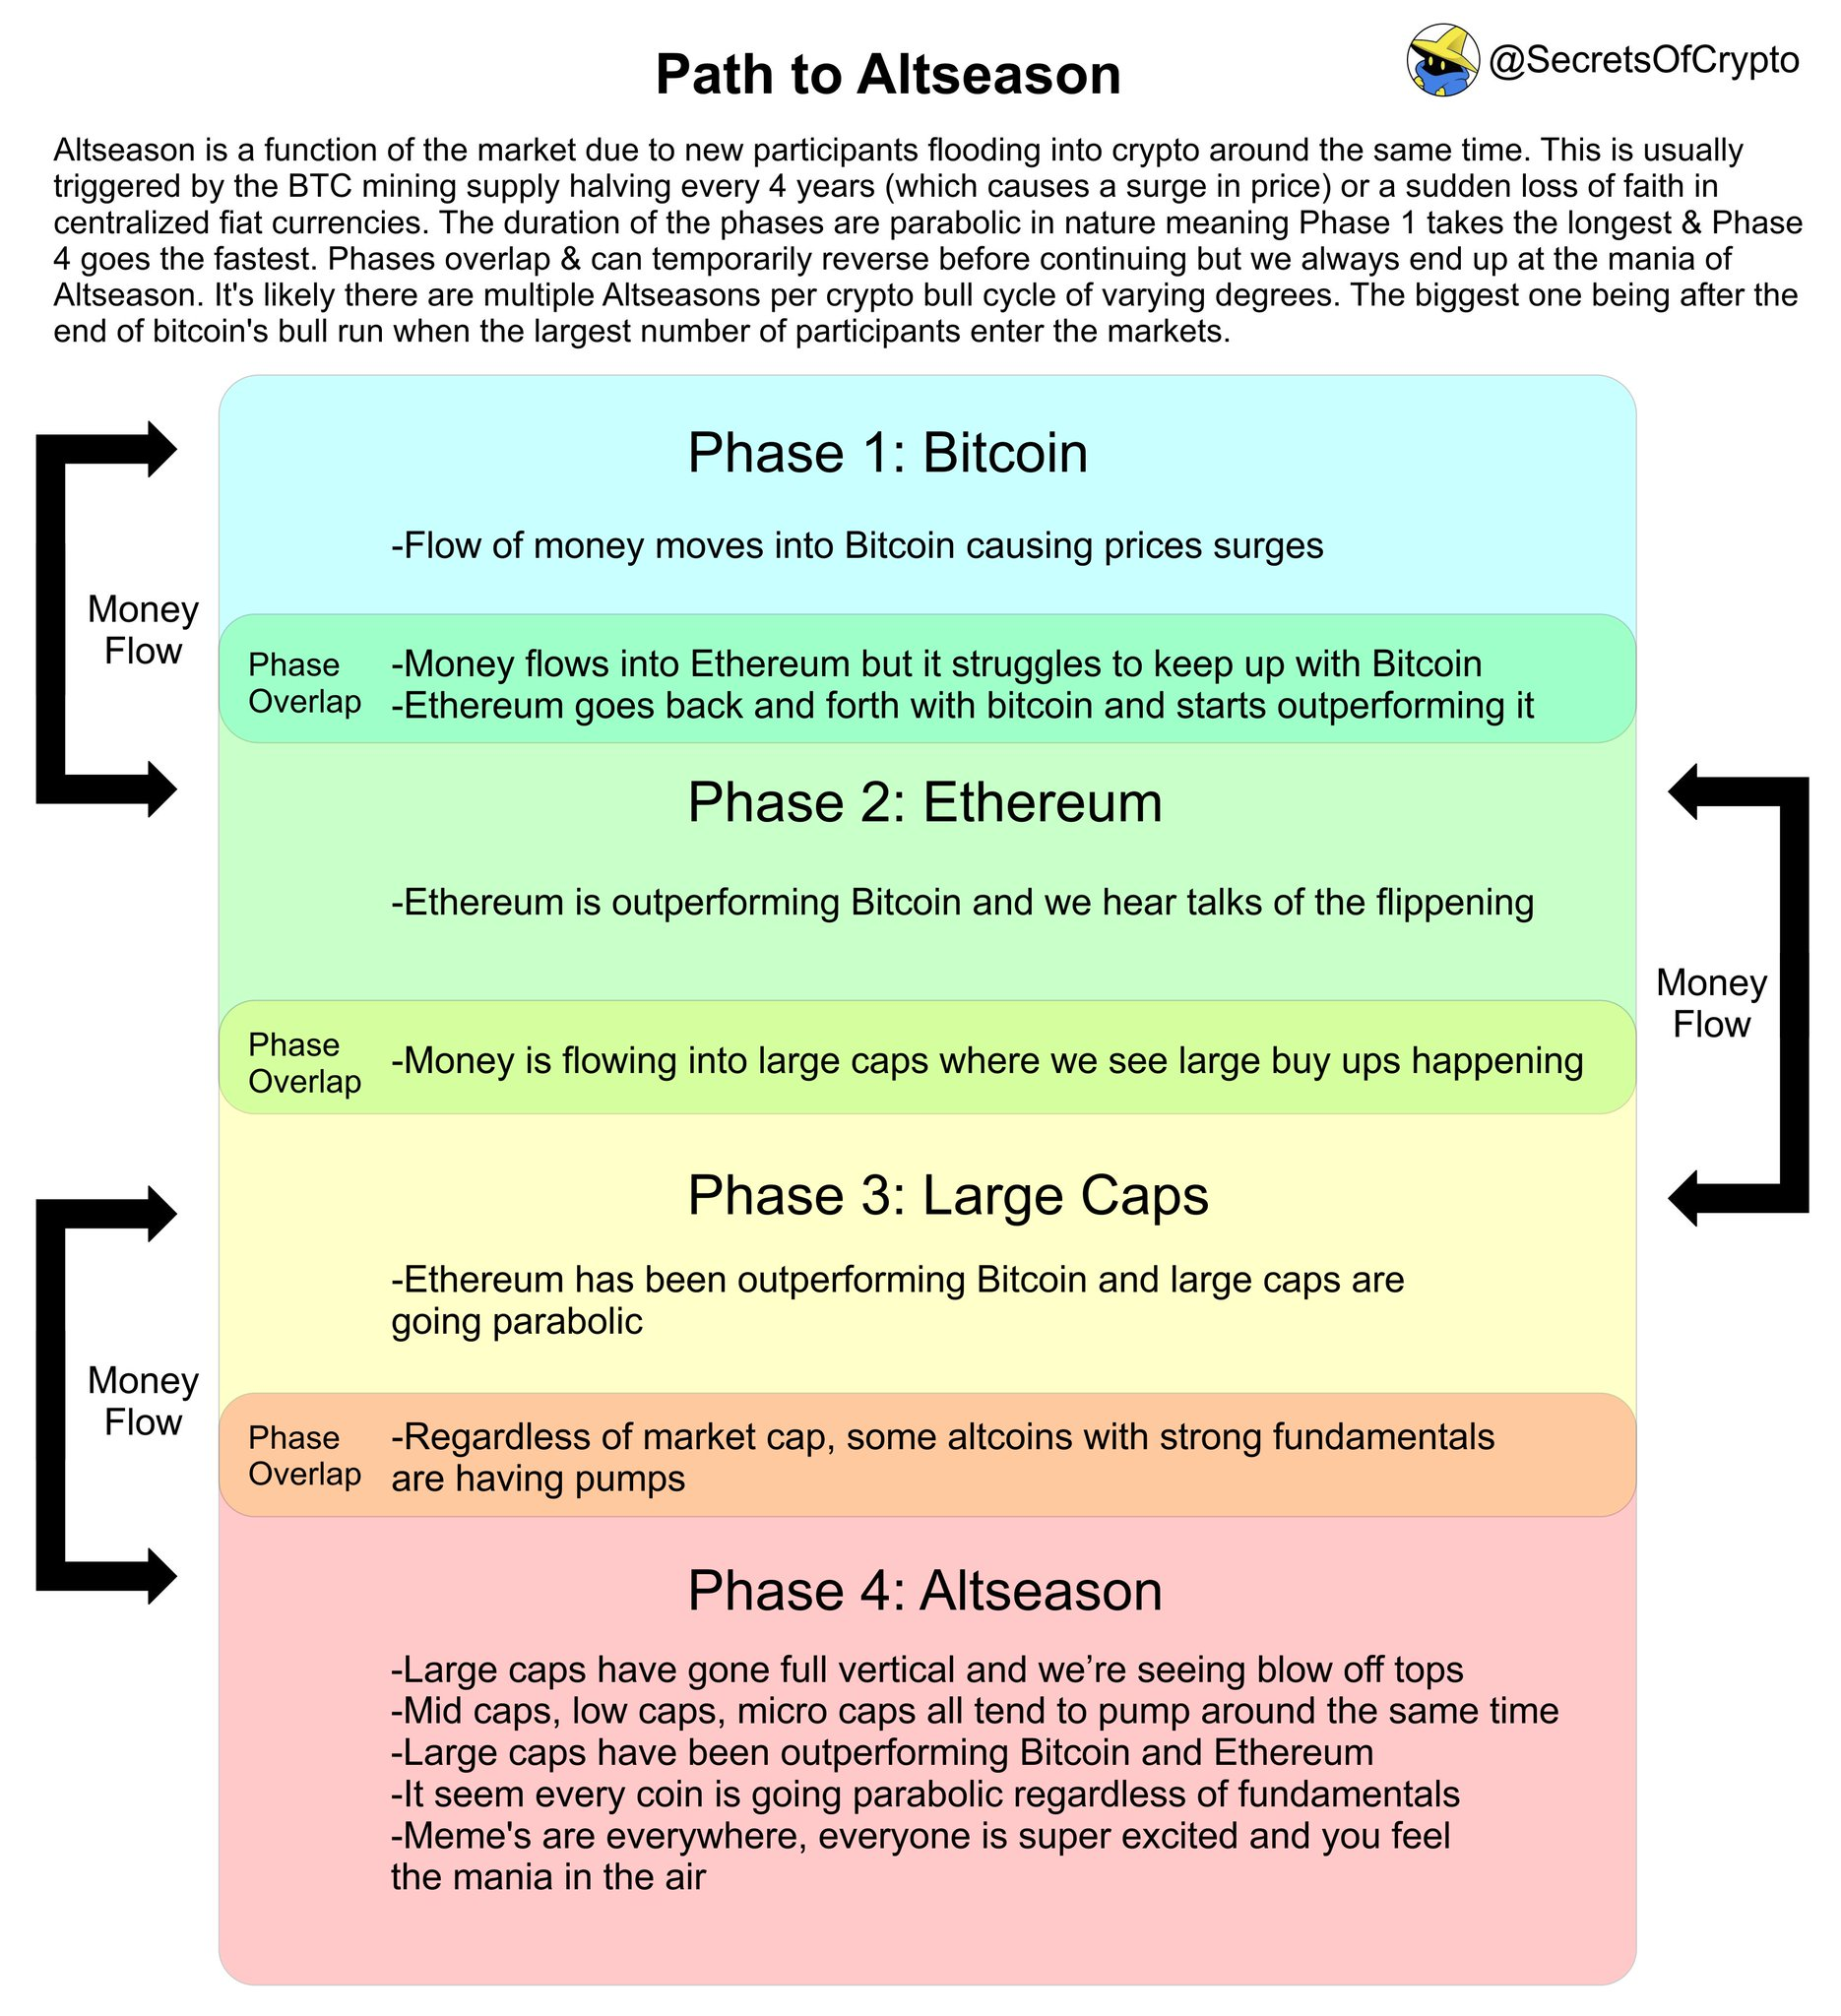
\includegraphics[width=0.5\linewidth]{path-to-altseason}

Bitcoin price action can cut this pattern short. Towards the end, a reliable signal for the top is when garbage coins pump across the board. 

\subsection{Dumb money vs smart money}
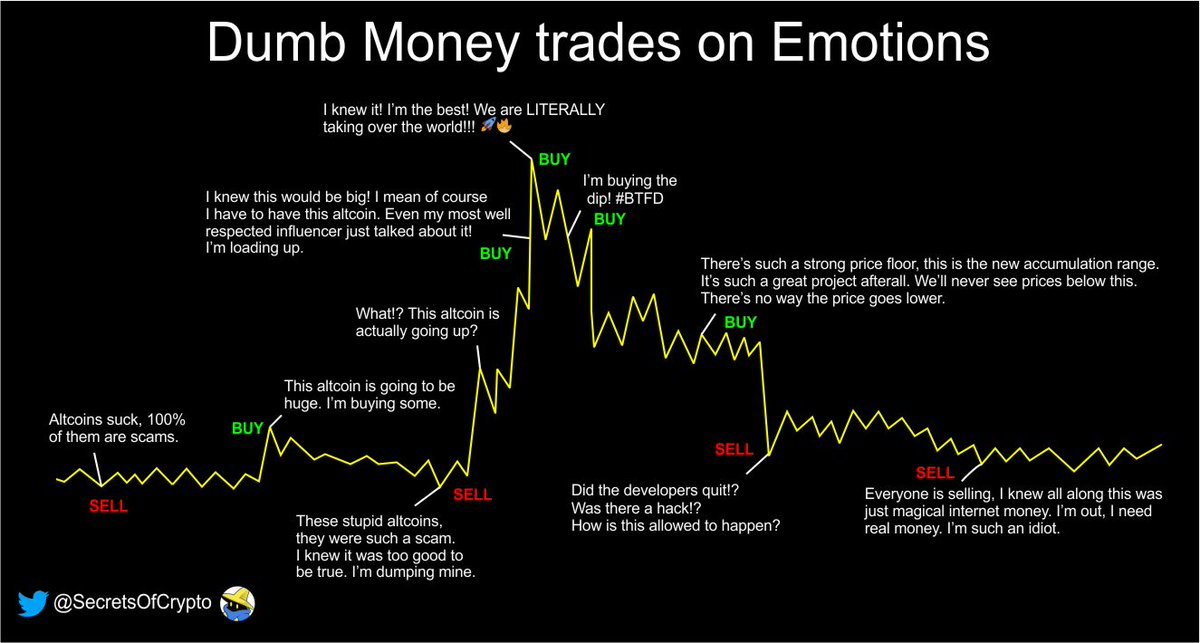
\includegraphics[width=0.5\linewidth]{dumb-money}
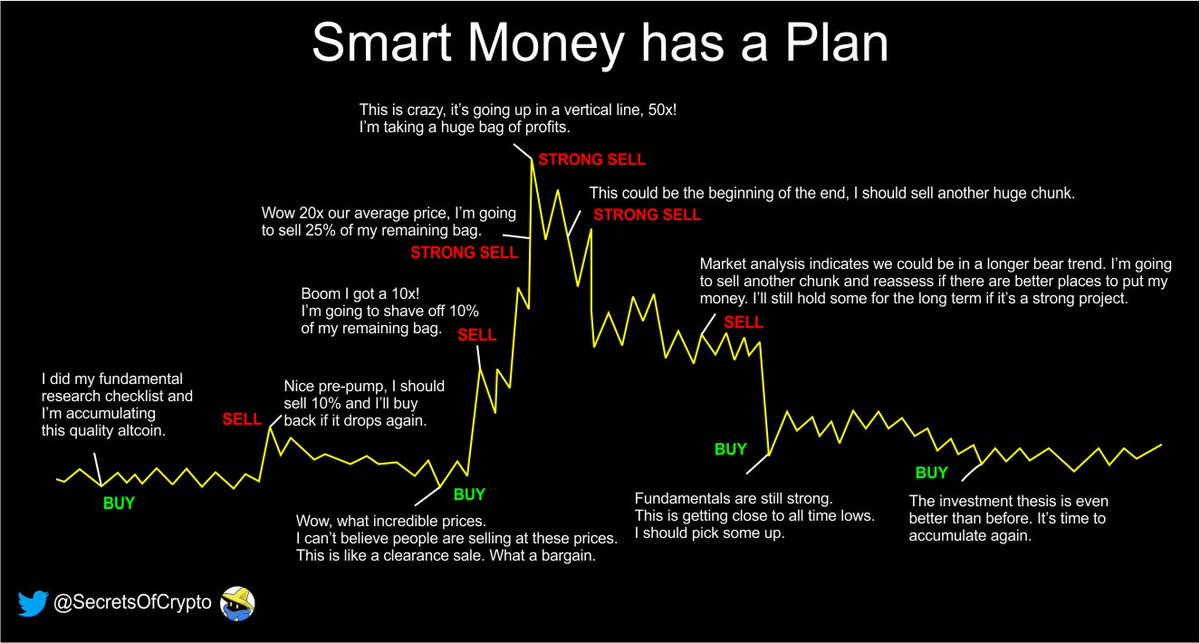
\includegraphics[width=0.5\linewidth]{smart-money}

\subsection{Flow of crowd for 4-year crypto cycle}
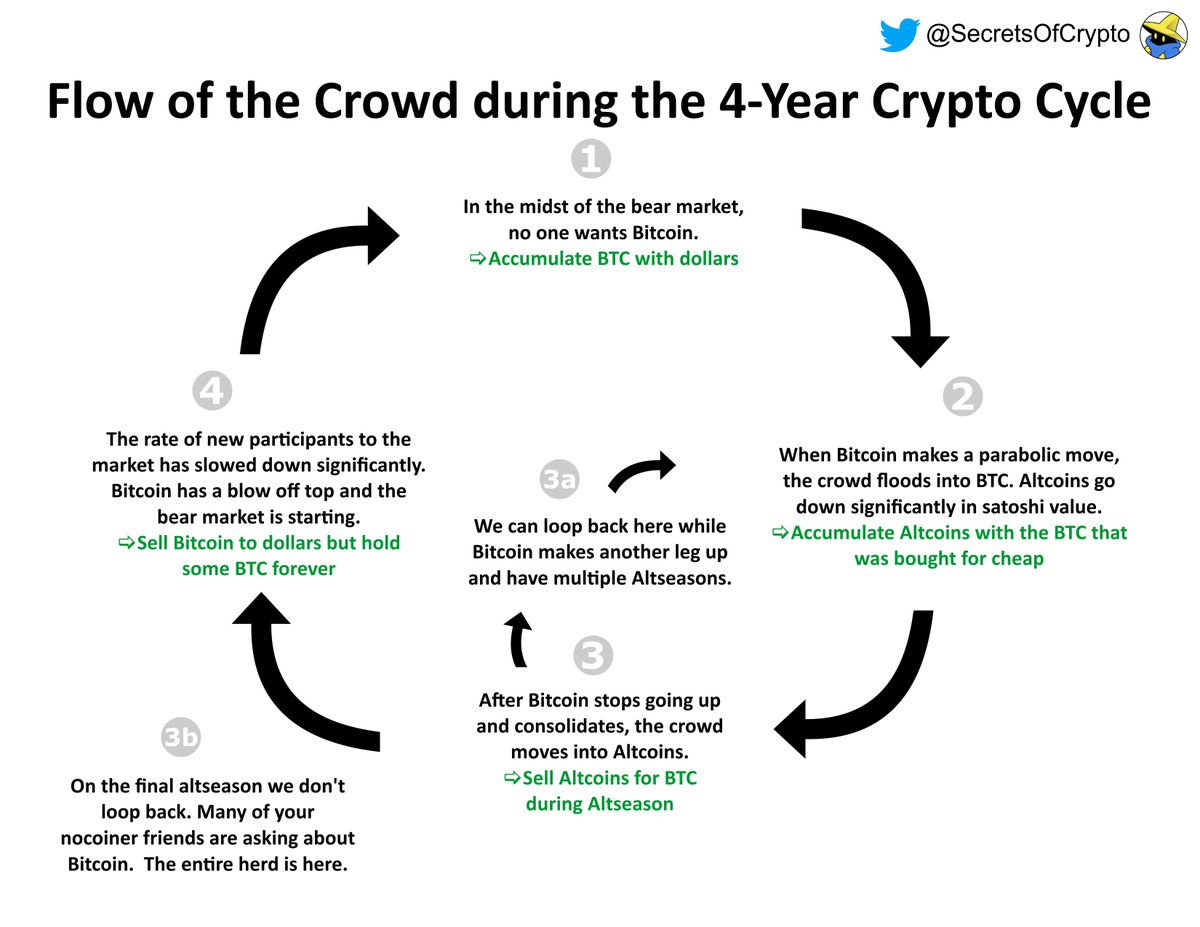
\includegraphics[width=0.5\linewidth]{crypto-cycle}
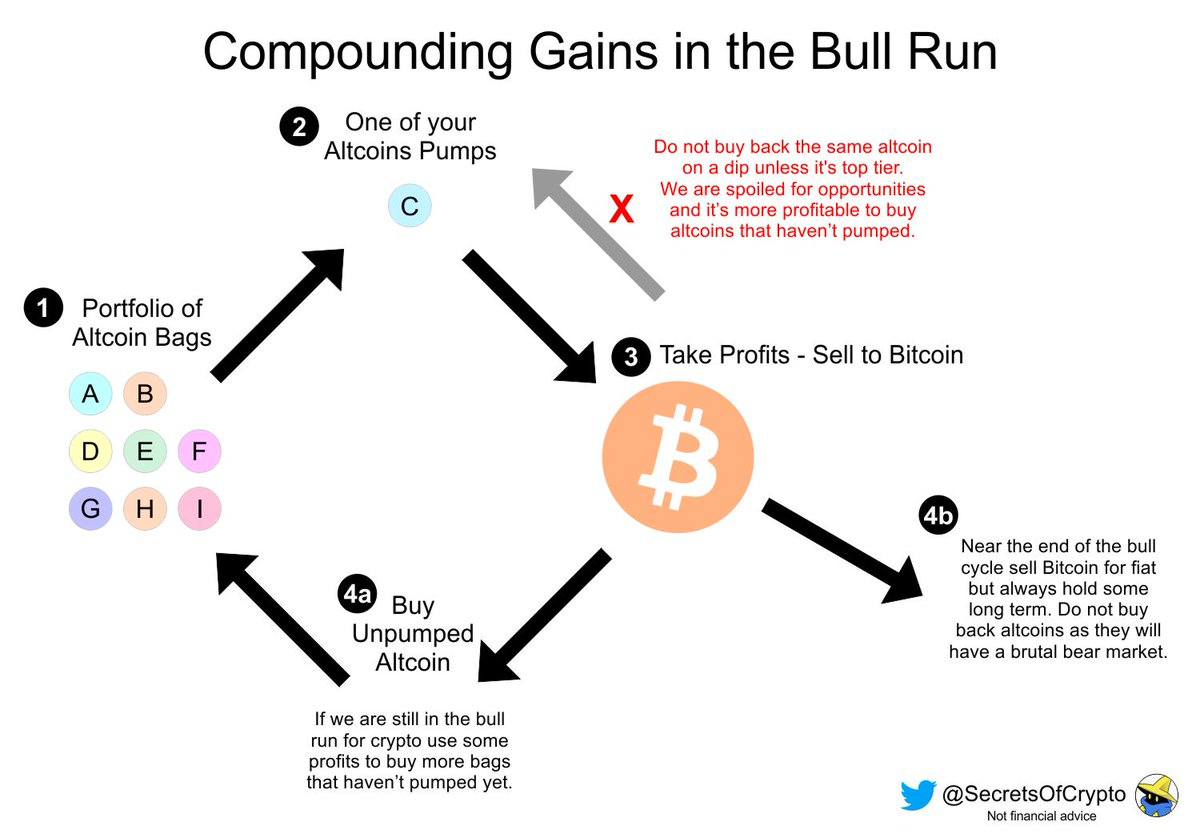
\includegraphics[width=0.5\linewidth]{bull-run-wealth}

\subsection{Altcoin Research Checklist}
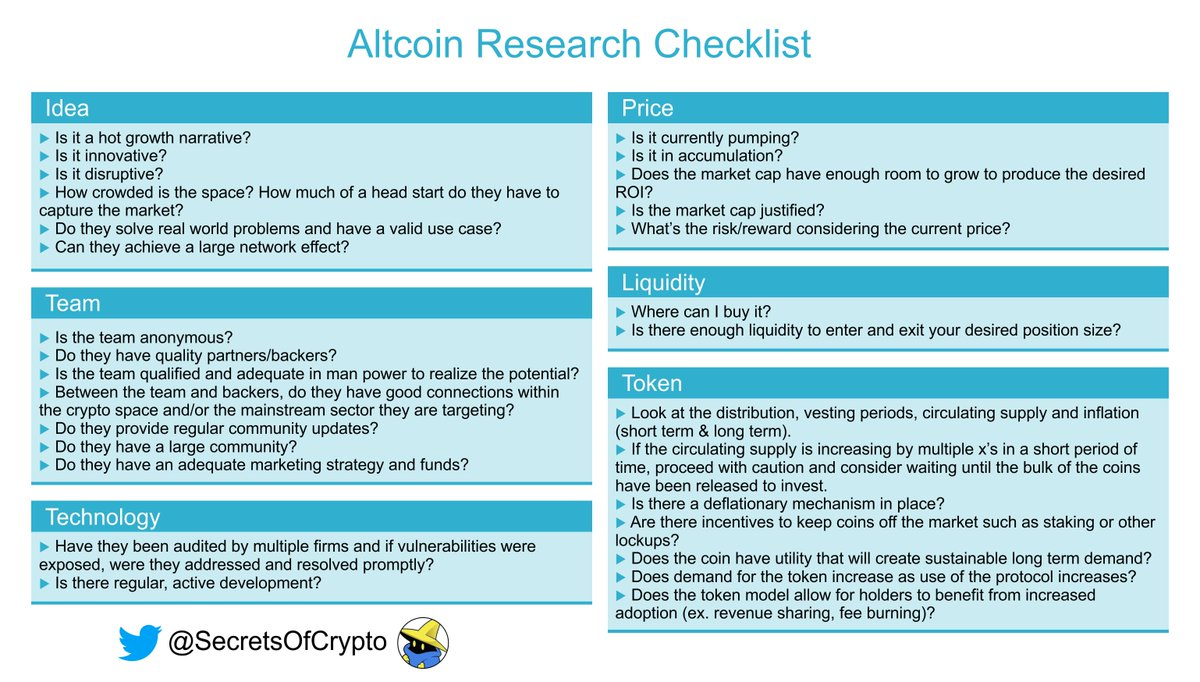
\includegraphics[width=0.6\linewidth]{altcoin-checklist}
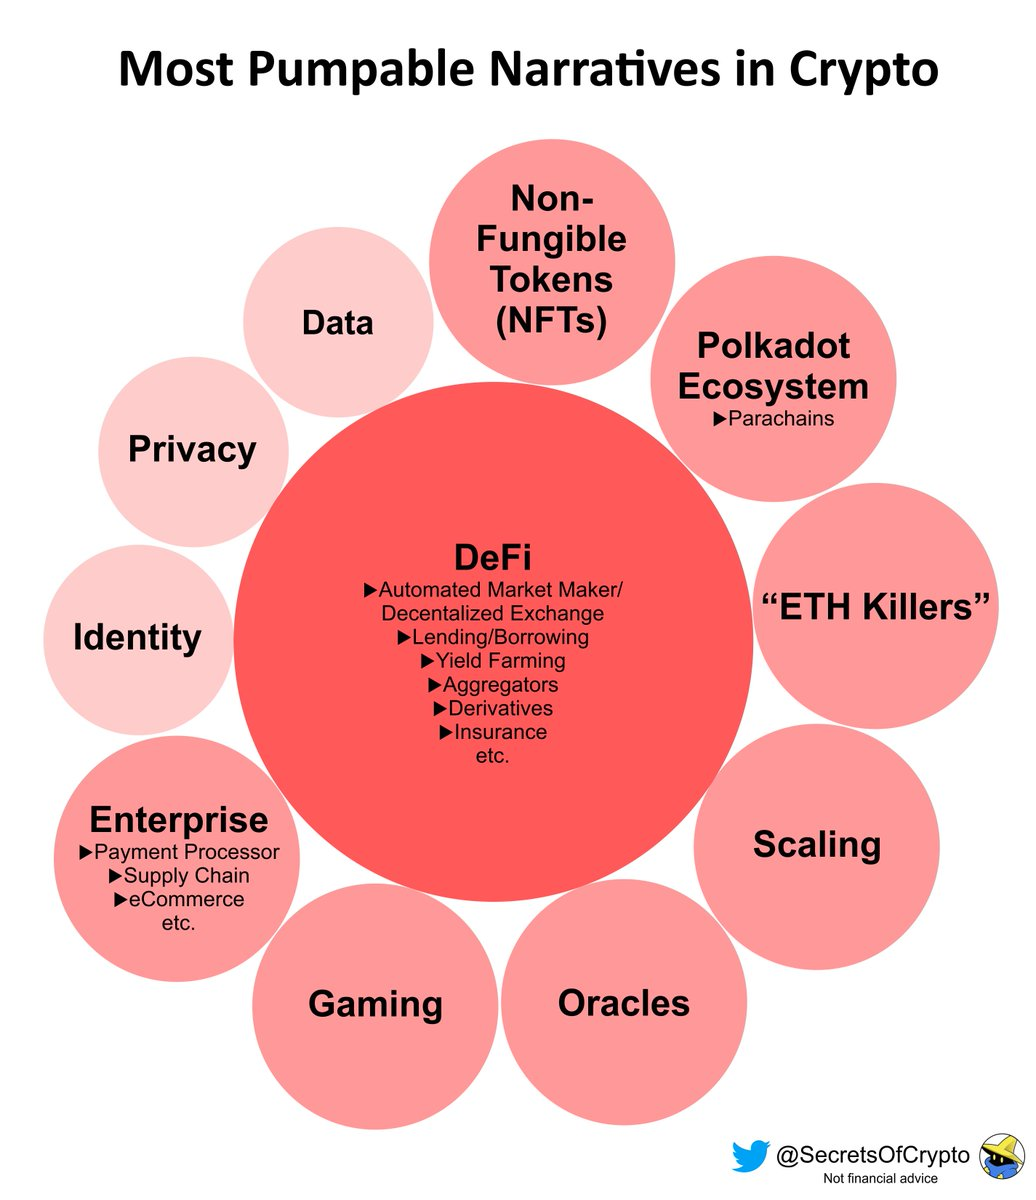
\includegraphics[width=0.4\linewidth]{pumpable-narratives}


\section{Copy-trading: We Like the Coins}
https://messari.io/article/messari-employee-holdings-policy-and-disclosures

Approx popularity: BTC, ETH, SOL, LUNA, HNT, RUNE, ATOM...Recommend rereading (page 19/165) their reasonings. May be very informative once I understand more. 

\part{People to Watch}
\section{Multicoin Capital}
https://multicoin.capital/

They've been right on The Graph, Helium, Arweave, Solana, etc. Try and keep up to date with their writings and videos. 

\section{Three Arrows Capital}
https://www.threearrowscap.com/select-investments/

\section{Bankless}


\part{Thoughts on Bitcoin}
Chances of the flippening is small (~20\% in 2022). BTC dominance is likely to continue falling. Meme coins are memes: they get old, and whey sht hits the fan and capital gains taxes come out people will sell. Privacy is a features, no need to invest in XMR/ZEC over BTC. Analogy to holding GE stock during dotcom bubble: even crashes are high above prices before dotcom bubble. Wrapped/synthetic bitcoin on other blockchains will double in 2022 (from 1.5\% of all BTC to 3\%, 75\% confident). 

\section{China FUD}
Chinese mining turned off: full recovery. No more hashrate FUD. Coal-powered bitcoin minders in China: Climate FUD done. 

But, predict that mining is legalized (70\% confident) in China due to geopolitics and clean energy stimulus. 

\section{Clean energy stimulus}
It's true, not just pro-bitcoin marketing. 

\section{Proof-of-stake vs proof-of-work}
Proof of work is still probably best for stateless money apps. Proof of work paved the way for proof of stake. PoS decentralization comes from thousands of interoperable PoS blockchains, each with own incentives and tokenomics. 

\section{The Bitcoin Roadmap}
Taproot upgrade in spring 2021 made bitcoin transactions cheaper and enhanced privacy defaults by making any transaction type look the same. 

\section{Lightning network in El Salvador}
Major success, will continue to 10x, but numbers are still small in comparison to ERC20 USD stablecoin settlements (\$200 million vs \$5 trilion)


\part{Market Infrastructure}
\section{Bitcoin Futures ETFs}
Are bad as long-dated contracts trade a higher prices to short-dated contracts. 

\section{CeFi vs TradFi}
We're not waiting for TradFi (the 'institutions': Goldman Sachs, CME, etc) to enter the space, they're being replaced by Crypto CeFi (Genesis, Binance, FTX, etc). It's over, we're beyond the point of no return. 

\section{CEX Ed}
God tier CEX: Coinbase, Binance, FTX. Keep an eye on Coinbase Wallet and DAO plans + upcoming NFT marketplace. Binance: super large, BNB gets 20\% of exchange profits. FTX: moves at super speed, plans to become an 'everything exchange' just like how Amazon became the 'everything store' by first selling books. 

\section{Bagholders (and stakers)}
Most TradFi entrants will choose hosted custody over self-custody, as a result Anchorage, BitGo, Fireblocks, etc, hit unicorn status as trad funds interest explodes. Reckon future will see 50-50 split between self/semi-custody vs checking-account style. 

\section{Payments Innovation}
Basically lots of innovation, Stablecoins; lots of companies hiring crypto teams, Visa bought a crypto punk. 

\section{CBDC}
Crypto fascist. Somehow really supports regulated stablecoins. Not sure if not familiar with UST or prefers USDC over possible future decentralized stablecoins. 

\part{NFTs and Web3 Plumbing}
Web3: paradigm shift towards a more democratized Internet and the chance to upgrade networks into crypto asset centered economies, and build systems where the incentives of network owners, network participants, and thirdparty developers are fully aligned. 

\section{Everything's coming together}
The 2020 DeFi boom supplied the “throughput infrastructure” of self-custodied, permissionless trading (like routing and bandwidth in Web1), which allowed NFTs to take off. The explosion of demand for NFTs (plus DeFi) pulled forward demand for more scalable Layer 1 and Layer 2 blockchains earlier this year. All of that will spur growth in DAO infrastructure in the new year: NFTs provide on-chain identity and reputation for DAO contributors; DeFi gives DAO members massive liquid pools of capital to govern; and scaling solutions will make on-chain governance economically feasible.

In Web3, cryptocurrencies and NFTs are the digital goods of the new economy, DeFi is the native financial system, Layer 1 networks are the rails that power everything, and DAOs are how the frontier gets governed.

\section{NFTs: Digital Goods on a global ledger}
Currently lots of hype and crazy valuations and are complete garabge, but will transform the world. NFTs are verifiably scarce digital property and potential is unlimited because blockchains become global transaction ledgers. 

\subsection{Million dollar jpegs}
Prediction: NFT market crash would be worse than 2015 bitcoin bear but trajectory of overall market will be the same: 100x+. Winning long-term plays are infrastructure related

\subsection{PFPs: Punks vs Apes}
Profile pictures: people buy because (1) got in early, (2) speculating, (3) trying to gain attention. If buy in, recommend not looking as an investment, rather as a consumable luxury good. Problem with NFTs being the entry ticket to a community is it suffers from the social token paradox and does not substitute meaningful club history or reputation. 

\subsection{Fan Tokens}
Win and help win is a good model. Fan tokens either fungible or not can be what helps crypto come into mainstream adoption.

\subsection{Axie Infinity and Play-to-earn}
Gaming so dominant in entertainment industry because of new mediums (streaming and freemium games). Crypto in gamining's revenue generation is mind-melting. Prediction, top gaming studios enters crypto in a meaningful way else threats posed by inaction will hurt. 

\subsection{Looted: Composable NFTs}
Word list NFTs. Something like abstract classes/interfaces where every game builds an abstraction to incorporate them in a meaningful way. 

\subsection{NFT Financialization}
Using NFTs as collateral. Fractional ownerships of nefts. These exist in the real world: timeshares, subletting in real estate, etc. 

\subsection{OpenSea \& Friends}
OpenSea success, Coinbase entering market, FTX already here with Gemini, and GameStop is also entering. OpenSea is NFT infrastructure

\section{The Cryptoverse}
Seven qualities:
\begin{enumerate}
    \item persistence: permanent, always gloabl hangout
    \item liveness: real-time just like in-person
    \item uncapped user 'presence': a stadium vibe
    \item economic robustness: NFTs are the goods, fungible tokens are the currencies and commodities
    \item relevance across digital and physical worlds: no walled gardens
    \item interoperability: portable goods, identities, IP
    \item user-driven evolution: content and experiences are created curated openly vs through a central company
\end{enumerate}

In the metaverse, it will be technically and socially impossible to 'right click save' NFTs as everything is all seamlessly tied to blockchain. 

\subsection{Metaverse and Meta}
Though cringe and can scoff at, they are pouring billions of dollars into this industry and can literally brute force their way to success. 

\subsection{Non-Fungible Credentials: Your Modular Identity}
Imagine NFT diplomas, composed of smaller tasks each composed of even smaller ones (like pass test\#1 NFT). Prediction: move towards meritocratic earned NFTs. In future, you crypto wallet can be universal digital identification. 

\subsection{Namespaces \& Data Sharing}
Decentralized domain name services. Trust decentralized ENS vs centralized Verisign who manages 85\% of world's 200 million websites?

Less than 1\% of world's data is used and analyzed. Web3 protocals like Ocean provide wrapper for these data packets by encouraging publich sharing and secure monetization of data. Addressable market is FAMGA's ad revenue. 

\subsection{DeSo Lotteries}
Decentralized social networks. Currently many upstarts (Bitclout, BlueSky, gm.xyz). Core concept: reward users that go 'viral' financially. 

\section{The physically decentralized (permanennt) web}
Physical survival of crypto in any industry requires decentralization of hardware. 
\begin{itemize}
    \item IPFS: decentralized system that allows any node to store data for a limited time
    \item Filecoin: incentivized storage network built on IPFS
    \item Arweave: long-term storage with own blockchain
    \item Sia: on-demand storage with own blockchain. 
    \item Filebase/Pinata: decentralized storage aggregators
\end{itemize}

\subsection{Physical Network Scaling}
\begin{itemize}
    \item Helium: very strong performer which bootstrapped hard hardware business model with right user economics
    \item Livepeer: decentralized video transcoding protocol gains traction due to rapidly growing video network
    \item Akash: stores docker containers at significatly reduced cost to cloud providers
    \item Andrena/Althea (pre-tokens) tackling internet service provider layer by enabling communities to set up hotspots and antennas that bring internet access to nearby towns
\end{itemize}
Livepeer on Eth, Ahash, Helium, Arweave on own blockchain: cetain multichain future.

\part{DeFi 2.0}
\section{USDT Bridge}
Unlikely of a Tether fail to put end to bull market. If USDT dies, much more likely comes at the hands of US Government seizure than bank-run. USDT is the bridge that gaps legacy finance to crypto, even if it's a rickety and shady rope bridge. 

\section{DAI vs UST}
There's room for both. DAI is the undisputed leader for Ethereum as it's 4 year trackrecord is hard to replicate for UST, but is mostly isolated on Ethereum whereas UST is rapidly expaning to other blockchains. Although momentum for UST is accelerating as it becomes defacto interchain stablecoin, MakerDAO currently holds an all time high TVL of \$20 billion and all growth for DAI has been organic. But unlikely one will replace the other. 

\section{The Algorithmic Stablecoin Renaissance}
Two new innovations: fractional reserve stablecoins and protocol controlled value.

\subsection{How an algorithmic stablecoin works}
Balance between two assets, one a stablecoin, and when stablecoin's price rises, new ones are minted, and likewise burned when price of stablecoin falls. The non-stablecoin asset absorbs the volatility. But has two limitations: (1) downward reflexivity can create 'back runs' on these protocols, and (2) lack of collateral means 'bank run' can go to 0. 

\subsubsection{Fractional reserve stablecoins}
Frax Protocol: balance between algorithmically backed stablecoin while also having 'perfect' amount of fiat in reserves. 

\subsubsection{Protocol controlled value}
Fei Protocol: Decentralized bank where protocol owns user deposited assets not liquidity providers (LPs), and can do with those assets however it wants (like using DeFi). 

\section{Emergence of Non-Pegged Stablecoins}
Not sure if Bitcoin will ever achieve stability given inflexible supply: in 2021 May plunged 30\% in one day even though at 750 billion market cap. Olympus DAO: issues own stablecoin, stabalized by it's reserve of assets (BTC, ETH, etc), just like how central banks stabalize their own currencies with reserve assets (USD, gold, etc). Rightful to be suspicious, unsure how these would hold up in a bear market, but may be the best bet for depegging crypto from the US dollar. 

\section{Worldcoin's Steely Gaze}
Impressive backers and audacious goal: fair launched digital currency for 1 billion people. It sounds sus, and there's probably mamy unknown-unknowns if this experiment is successul. 

\section{Uniswap v3 vs the world}
Some think Uniswap would subsume all other Eth DEXs. V3 essentially allows limit orders and allows liquidity providers to adjust their ranges of buy-sell liquidity, allowing for 'concentrated liquidity', which is the future. 

\section{Perp vs dydx}
Battle to watch: DeFi perps vs CEX perps. 

\section{The Alchemix of DeFinance (2.0)}
\subsection{Crypto hype and installation cycles}

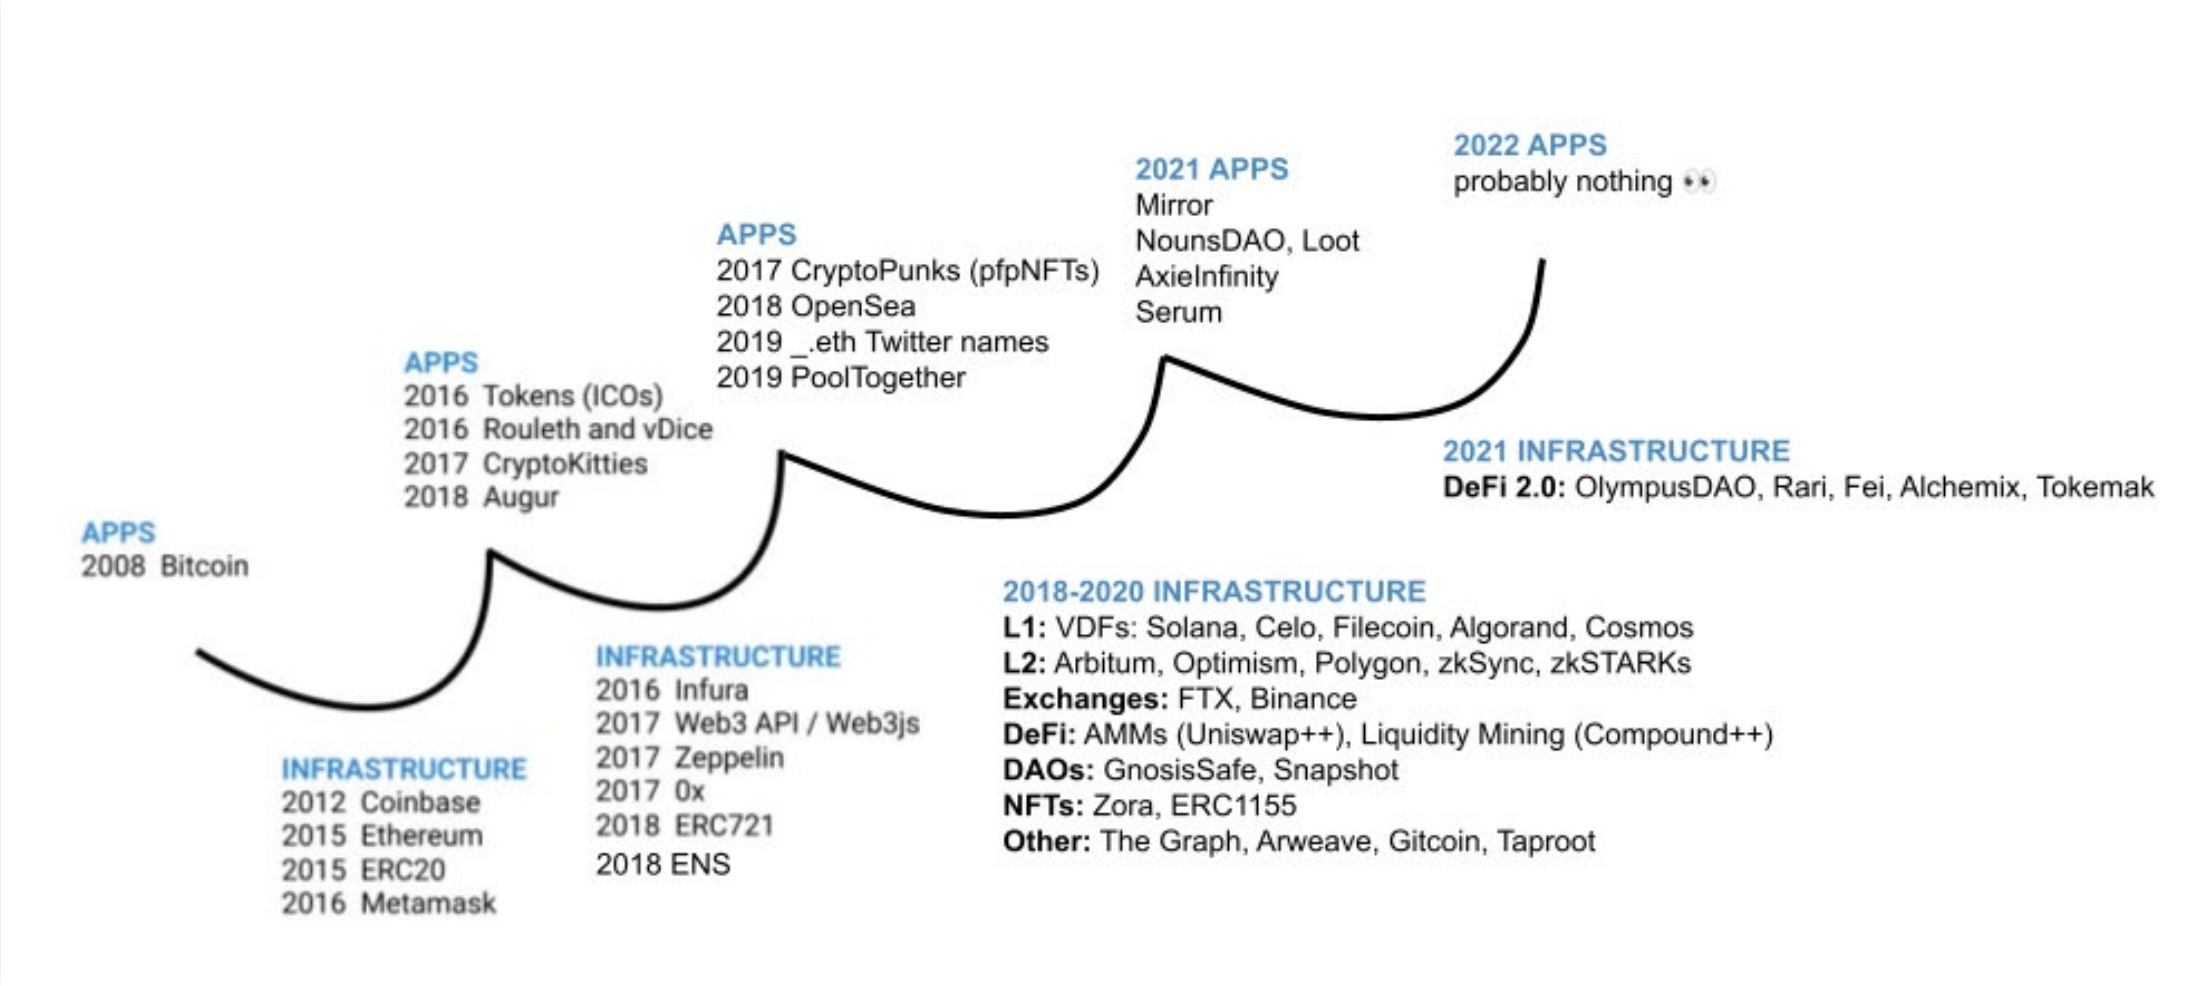
\includegraphics[width=0.8\linewidth]{crypto-hype-install}

\subsection{DeFi 2.0}
Yield farming 1.0 was unsustainable as LPs provided capital is 'hot' and moves from protocol to protocol with greater risk-adjusted returns. Instead of issuing native treasury token yield farms, create 'liquidity as a service' scheme that rents liquidity from other protocols. 

\subsubsection{Olympus, Tokemak, and Fei}

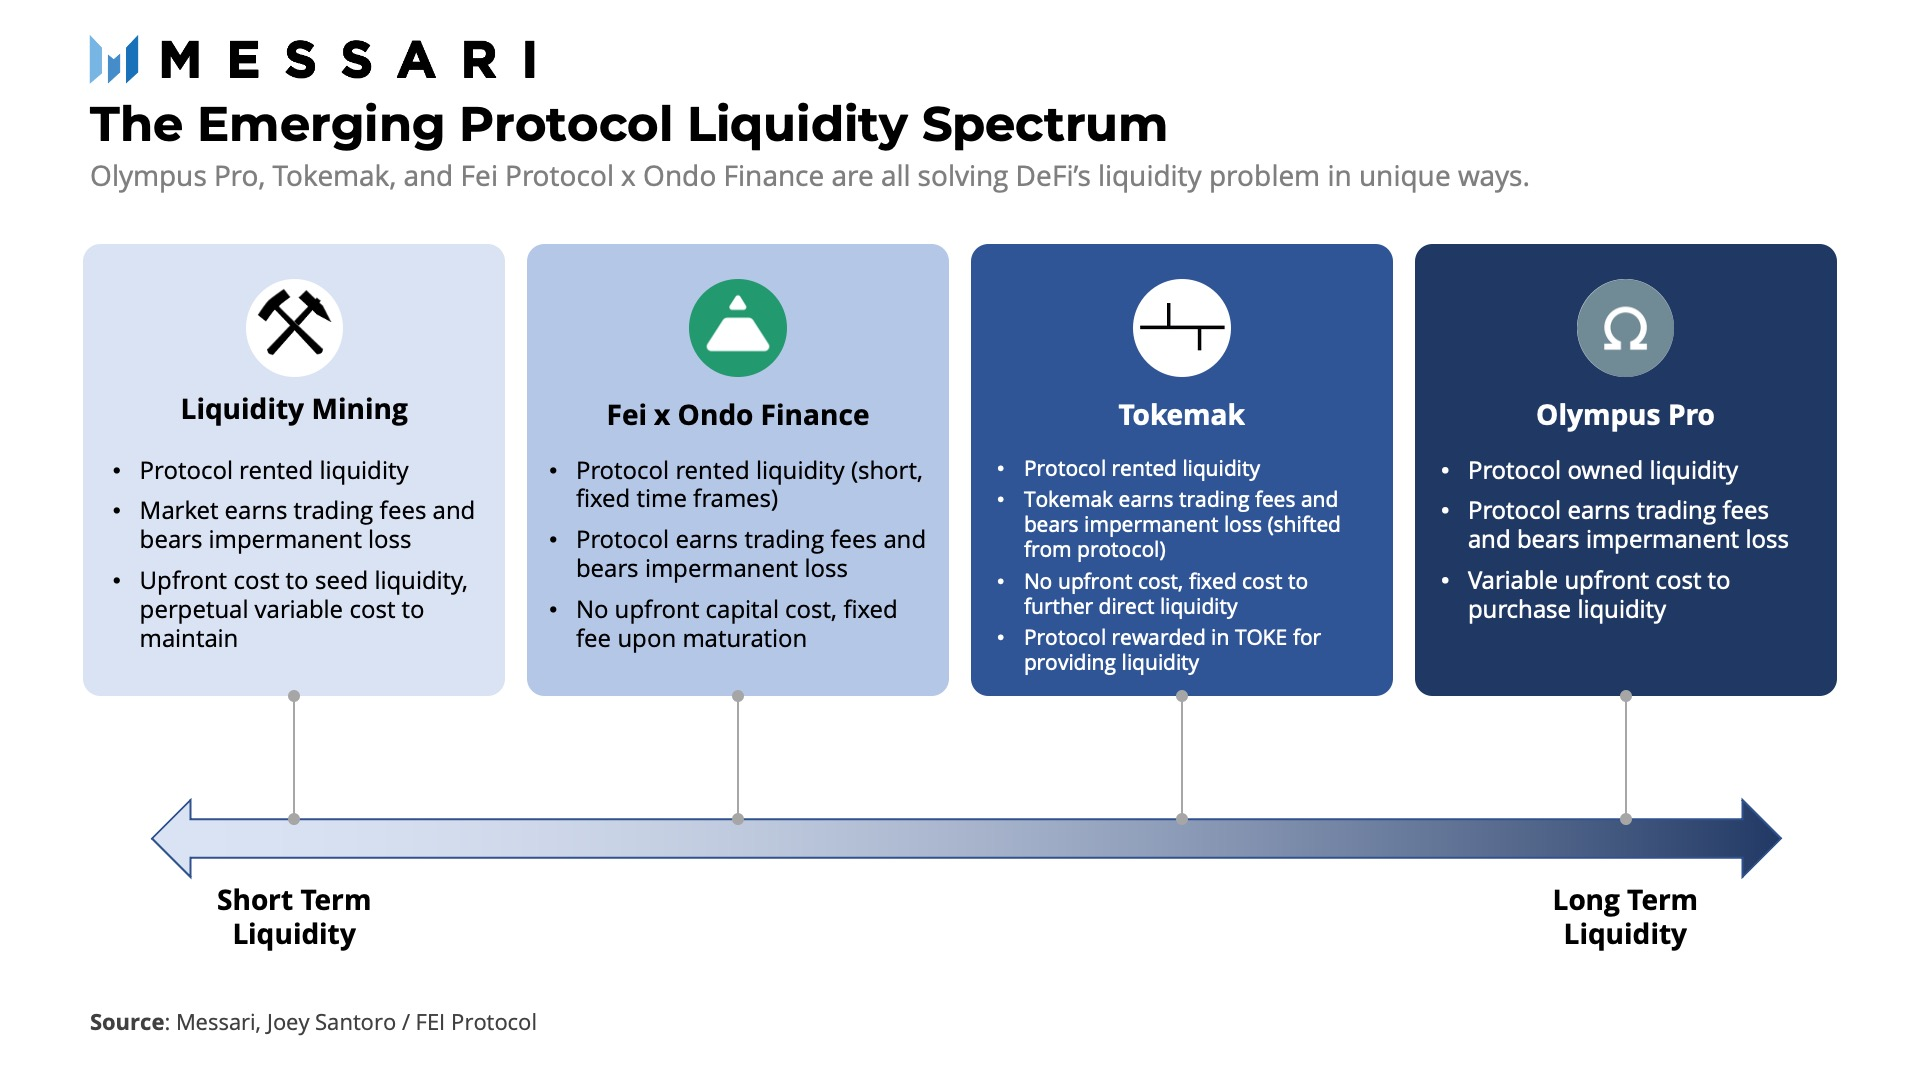
\includegraphics[width=0.8\linewidth]{protocol-liquidity-spectrum}

\subsection{Protocal controlled value}
Protocol controlled liquidity is a subset of protocol controlled value. If protocol controlled liquidity is about DAOs provisioning liquidity using their token treasuries, protocol controlled value is about DAOs monetizing their balance sheets more broadly.

Olympus DAO now has a treasury worth more than \$700 million in non-native assets, and is putting those assets to work in DEXs, lending protocols, yield aggregators, and even venture capital. That improves the returns of the DAO (its treasury assets generate yield) and reduces its cost of capital (the DAO doesn’t pay external sources for its liquidity). Higher revenues. Lower costs. This is the biggest unlock of DeFi 2.0.

Beyond new models for liquidity provisioning and balance sheet monetization, this year has brought the dawn of “automaters”, “enhancers”, and “extenders”. Automation protocols rebalance liquidity positions across AMMs and Layer 1s, recycle rewards, and provide “auto-compounding” services. Convex Finance is one the leading examples - they “recycle” \$CRV and Curve LP tokens for boosted rewards, trading fees, and governance tokens.

Enhancers are protocols that do not introduce new operating models for DeFi, but rather recycle the outputs from existing protocols to optimize returns for the end user. A good example of this is Abracadabra.money, which is similar to MakerDAO but with the important difference that it creates CDPs (collateralized debt position) from yield-bearing assets (and has much looser risk controls).

Extenders are protocols that stack various underlying DeFi protocols. Alchemix is a good example. It’s vaults function similarly to MakerDAO’s, but the protocol also rehypothecates its collateral assets and deposits them into yield aggregators like Yearn, creating yield generating synthetic tokens which look like “self-repaying loans.” The rehypothecation creates risk, as the protocol absorbs the risks of the lower-level protocols it’s built on. Still, self-repaying loans!

Critics will point to subprime mortgages and other derivatives, and note that “DeFi 2.0” will have a significant garbage in, garbage out problem, with cascading failure risks. Others will greedily (and literally) invest in the magic internet money (\$5 billion in liquidity in six months). I’ll be honest. I haven’t yet wrapped my head around all of this yet, and whether it’s all moon math or a new sustainable financial model.

\section{The Fat Application Thesis}
Multichain future here to stay: Crypto is going modular at an accelerating rate. Ethereum plans to rely on a roster of Layer 2 execution platforms like Optimism, Arbitrum, StarkWare, and ZKSync. Ethereum competitors like Solana and Avalanche have developed formidable parallel DeFi layers and user bases. Cosmos has unlocked cross-chain communication, bringing its multi-chain IBC universe to life. And Polkadot’s parachain auctions have finally kicked off.

An Ethereum-only strategy is not viable to capture most of crypto's growth in coming years because transactions on Layer 1s become uneconomical. 
\begin{itemize}
    \item Ethereum-centric: Protocols deploy copies of their contracts only to Eth Layer 2s like Arbitrum or Optimism (Uniswap)
    \item Spray and Pray: Protocols deploy copies of their contracts to any EVM-compatible chain or Layer 1 sidechain (Sushi)
    \item Targeted EVN Destinations: Protocols deploy copies of their contracts to EVM-compatible chains or sidechains once there networks have shown initial promise, often after a native liquidity mining program. (Curve and Aave)
    \item DeFi Hub (Independent Chain). Protocals launch a new standalone chain with potential to connect with multiple networks (Compound Chain)
\end{itemize}

Fat Application Thesis: Interoperability of state and value is likely to place downward price pressure on layer-1 blockchains that have no monetary premium, while enabling strong middleware protocols to achieve cross-chain, winner-takes-most dominance in their respective services.

Thesis has not yet materialized yet: (1) in month 16 of DeFi bear market, (2) infrastructure for seamless multichain usage is immature. But predict thesis to materialize in near future. 

\section{Tokenized Funds and Index Co-Op}
Little inovation in ETFs for years. Check out Bankless \$BED and \$GMI tokens

\section{DeFi's Split Personalities}
Though technically decentralized, developer teams have substantial control over frontend/application and can bend to laws and regulations (like Uniswap delisting some assets). Sia Skynet is trying to solve this with decentralized front-ends.

\section{The CeDeFi Boom}
Not sure if it's the future we want. 

\section{Governance Snafus}
Governance infrastructure still quite new but rightfully to be bullish. Many mistakes made in past, like Compound sending away \$160 million worth of tokens during routine protocol upgrade, etc. Bullish on infrastructure that leads to DAOs replacing most companies

\section{Security and the Dark Forest}
Three things to keep an eye on:
\begin{enumerate}
    \item Smart contract insurance (Nexus--first crypto insurance unicorn, and definitely not last)
    \item Verified secure smart contract libraries and security-as-a-service. (Forta)
    \item Perpetuity on smart contract security researched. 
\end{enumerate}

\section{Bullish Unlocks and FDV}
'Fully diluted value' is a bad metric for ecosystems managed by DAOs vs centralized foundations. FDV is max-supply market cap, and matters more in well-distributed tokens than ones with big, long-term backers.

\part{ETH, Layers, and Bridges}
\section{ETH's Q3 Earnings Report}
Check out Bankless's Q3 update on Eth. Now there's more value locked in DeFi than the marketcap of most banks. 

\section{The Merge and Liquid Staking}
JP Morgan projects staking will be \$40 billion/year industry in 2025. Liquid staking: create liquid synthetic representations of locked (staked) capital. Potential 50x, is invested in Lido and Anchor. 

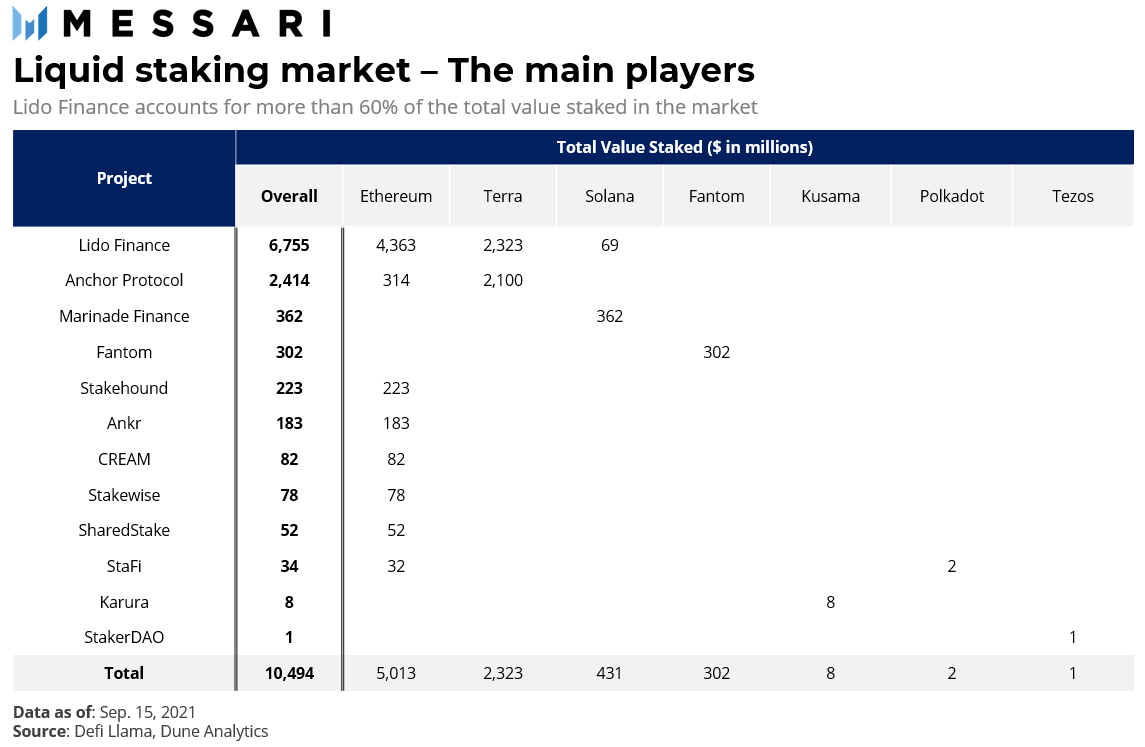
\includegraphics[width=0.7\linewidth]{liquid-staking}

Obviously very bullish cause can earn staking rewards and maintain liquid collateral, but there's bank-run risks when bull market is over. 

\section{To EVM or Non-EVM}
Major tech platforms trend to trend into duopolies: Windows vs Mac, Android vs iOS, Chrome vs Firefox, Intel vs AMD, etc. May expect to see similarities in crypto, even with multichain future. Upstart choice: EVM, or on a new tech stack that may not even survive a bear market. 

\section{Layer 1 Relative Valuations}
\begin{itemize}
    \item Decentralized and secure: Ethereum, Polkadot, Cosmos
    \item Fast and secure: Solana
\end{itemize}
When it comes to the relative valuations of these projects, it helps then, to think about the size of their entire economies, their developer ecosystems, the value they secure, the interoperability and incentives they offer, their value capture mechanisms, and which technical tradeoffs you believe the largest applications will choose to optimize for.

Also Eth is leaking value to rollup chains and non-EVM rivals. Eth sits at ~60\% dominance in L1s, but will likely fall below 50\% in 2022 or L2 rollup tokens will eat into Eth's growths. 

\section{Solana Summer Never Ends}
Executing at breakneck pace: \$100 million for decentralized social media with Reddit cofounder, \$100 million with FTX for blockchain gaming, Brave migration to Solana as default blockchain, etc etc. 

It is normal for networks to discover catastrophic bugs early in their lifecycles. 

\section{Polkadot's Slow and Steady Rollout}
Polkadot parachain auctions are kicking into high gear now. Inverting ETH 2.0 model: instead of apps fleeing Layer 1, Polkadot has L0 with generalized security and 'apps' as parachains. 

\section{Cosmos and IBC Opt-in}
Protocol is entirely open and independent of Cosmos hub, different from Polkadot and Ethereum. 

\section{Terraforming La Luna}
Terra UST gone from 0 to \$7.2 billion in first year. Mirror (Synthetic stock application) has \$1.5 bn locked value. Terra's Anchor protocol has nearly as much LUNA as ETH's Lido. 

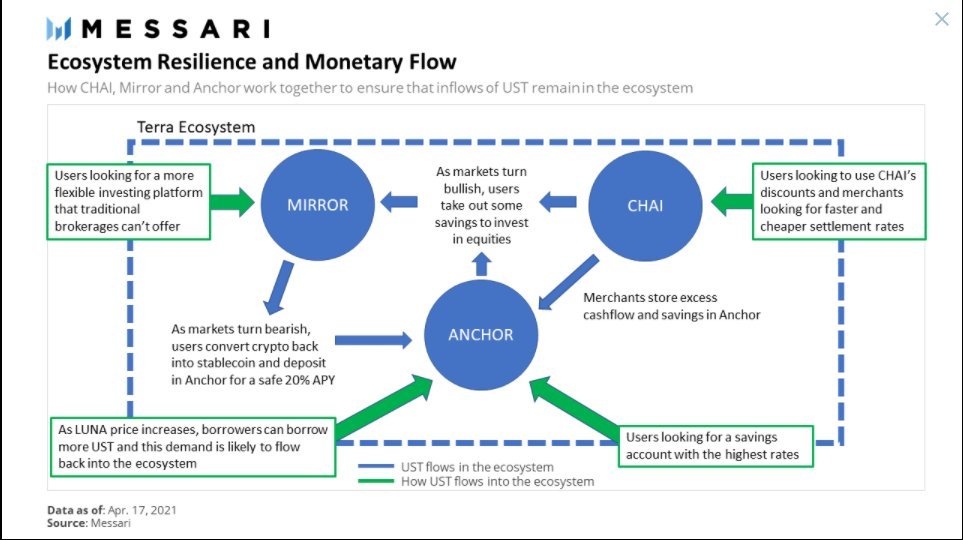
\includegraphics[width=0.75\linewidth]{terra-ecosystem}

Terra's biggest headwinds are known unknowns: (1) SEC vs Mirror for synthetic stock tokens, (2) reflexivity of UST and LUNA as primary source of collateral (had to take \$70mm infusion from Terraform Labs when stability reserves at Anchor were insufficient, and once when UST almost became insolvant when market cap of LUNA fell below UST). However, connection to Cosmos ecosystem (Columbus-5 upgrade) and ETH, SOL, and BSC via Wormhold v2 will derisk some of that reflexivity. Bullish on Terra's longterm potential. 

\section{The Best of the Rest (of the L1s)}
\begin{itemize}
    \item ADA: No one recommends replacing portfolio allocation on SOL, DOT, LUNA, ATOM with ADA. 
    \item ALGO: made some moves
    \item FTM: worked on by Yearn founder
    \item Near: aggressive on grants incentives and expanded ecosystem through EVM compatible Aurora sidechain
\end{itemize}

\section{Polygon Flippens ETH}
Seven paths to L2 scaling:
\begin{itemize}
    \item Layer 1 optimizations
    \item Layer 0 interoperability: Eth 2.0, DOT, ATOM all make similar assumptions that their networks will be networks of interoperable chains with shared settlement layers
    \item Payment Channels: Lightning network. Lock payment in a channel and can operate with other channels that use same scripts. Only good for payments
    \item Sidechains: xDai. BSC arguably sidechain of Eth. Plug into some L0/L1 network but are responsible for own consensus security models. 
    \item Plasma: effectively dead, essentially copies of eth anchored to eth. 
    \item Optimistic Rollups: Optimism and Arbitrum. Mini blockchains that move computation off eth. They separate state storage (full transaction data-stored in rollup chain), and fingerprint of that state (pushed to L1), and 'optimistically' assume fingerprint represents correct transaction history on the rollup. Since Eth stores fingerprint, serves as final arbiter of truth. 
    \item ZK-rollups: zkSync and StarkWare, dydx uses StarkWare. Are fast because uses 'validity proofs', making them instantly varifiable and eliminating need for liquidity-sucking challenge peiod. EVM-compatible solutions aren't live yet. 
\end{itemize}

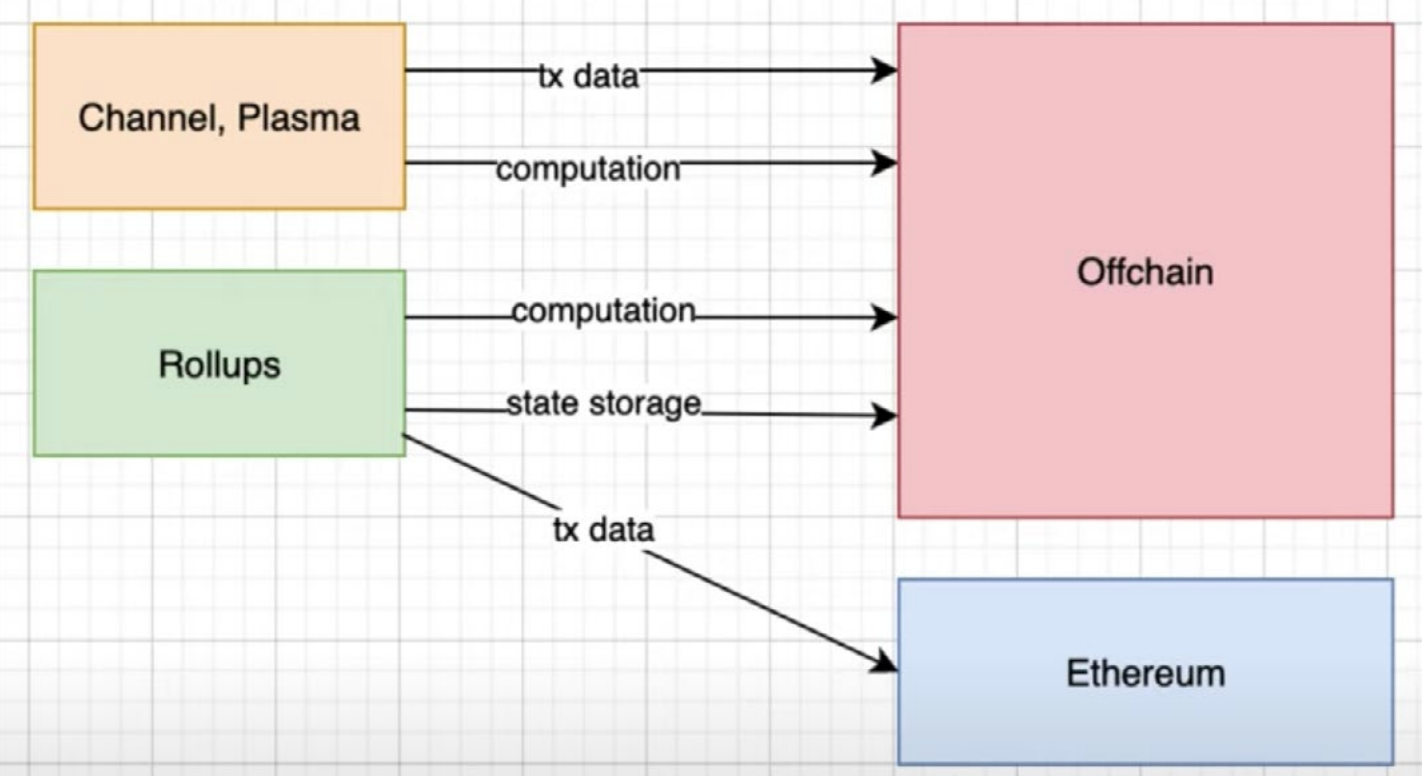
\includegraphics[width=0.6\linewidth]{scaling-solutions}

\subsection{Polygon}
Recently flipped eth with active user addresses. Recently launched Polygon SDK, a framework for launching new blockchains that serve as a rollup or standalone chain. On long-enough timeline, all crypto will converge to zero-knowledge crypto

\section{They're Optimistic and Zero-knowledge}
Eth rollup-centric design for eth scaling looks similar to DOT and ATOM: independent EVM-compatible execution-layer blockchains that rollup to same Ethereum Beacon Chain picking up steam between optimistic and zero-knowledge. 

\section{Build me a bridge}
Likely even more blockchains rist in coming years with the launch of layer 2 rollup chains. Blockchains starting to resemble physical world today: defined by nations where each have their own economies with own rules. However currently, isolationist, hard to move value between. Cosmos and others solving this problem

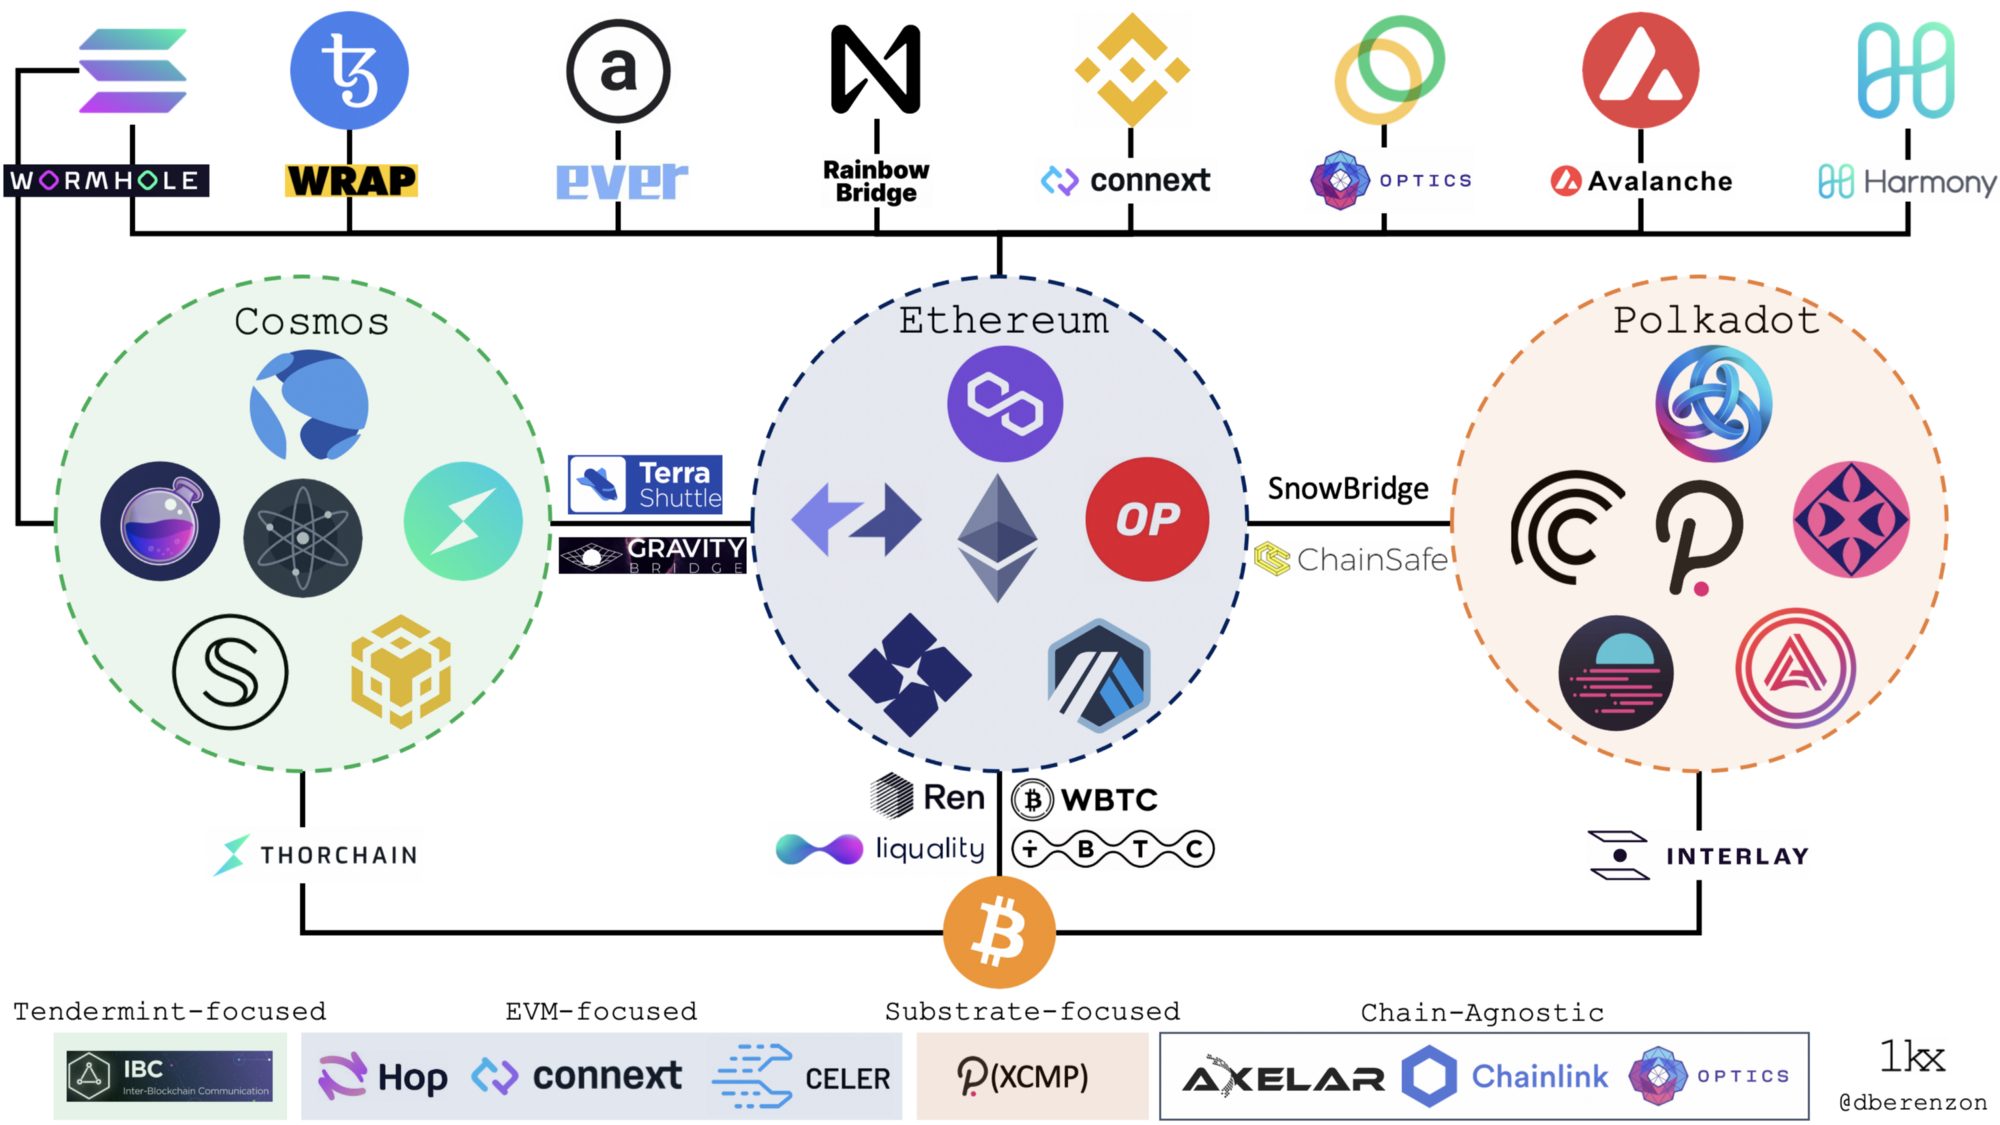
\includegraphics[width=0.7\linewidth]{interoperability}

Just as Ethereum’s composability enabled developers to package protocols together and build new dynamic applications (e.g. Yearn depositing assets into Compound, Aave, Curve, etc, for automated yield), we’ll likely see similar cross-chain applications that emerge once the bridge infrastructure is ready and capable of unlocking crypto collateral.

Cross-chain interoperability is also likely to standardize around a small number of trusted, widely integrated protocols. The immaturity of today’s solutions creates significant user and developer friction, but a bridge that’s credibly decentralized, battle-tested, and well-integrated across Layer 1s would likely emerge as the preferred choice for cross-chain liquidity simply due to its predictability and reliability. As the multichain economy grows, it’s inevitable that cross-chain bridges will facilitate an enormous amount of asset and data transfer volume.

Prediction: the most popular L1 <> L2 / L1 <> L1 / L2 <> L2 bridge protocols will have higher daily volumes than the most popular centralized exchange within five years.

\section{Wrapping it all up}
Time will tell if the markets are overheated in the short-term, but we’re just getting started in the crypto supercycle.

\part{The DAO of DAOs}














\end{document}
